\documentclass{article}
\usepackage[utf8]{inputenc}

\title{Korisni alati na androidu za učenje programiranja}
\author{Luka Nedeljković,Danilo Nikolaš,Nemanja Kelečević }

\begin{document}

\section{Android Studio}
Android Studio je jedan od najzastupljenijih i najbitnijih alata za Android programere. To je \textbf{integrisano razvojno okruženje} (IDE) za Android, zasnovano na softveru JetBrains IntelliJ IDEA. \\
Službeni programski jezik je Java, ali su takodje podržani C++, a i od nedavno Kotlin. Razvojno okruženje poseduje kompajler koji omogućava stvaranje APK datoteka, XML uređivač, kao i funkciju za "prikaz dizajna" pomoću koje vizuelnim putem omogućava organizovanje elemenata na ekranu. \\
Android Studio nudi kompletan set dodatnih alata koji programeri mogu efikasno da iskoriste, kao što su AVD Manager, Android Debug Bridge, monitor za praćenje performansi itd.\\

\begin{figure}[ht!]
    \centering
    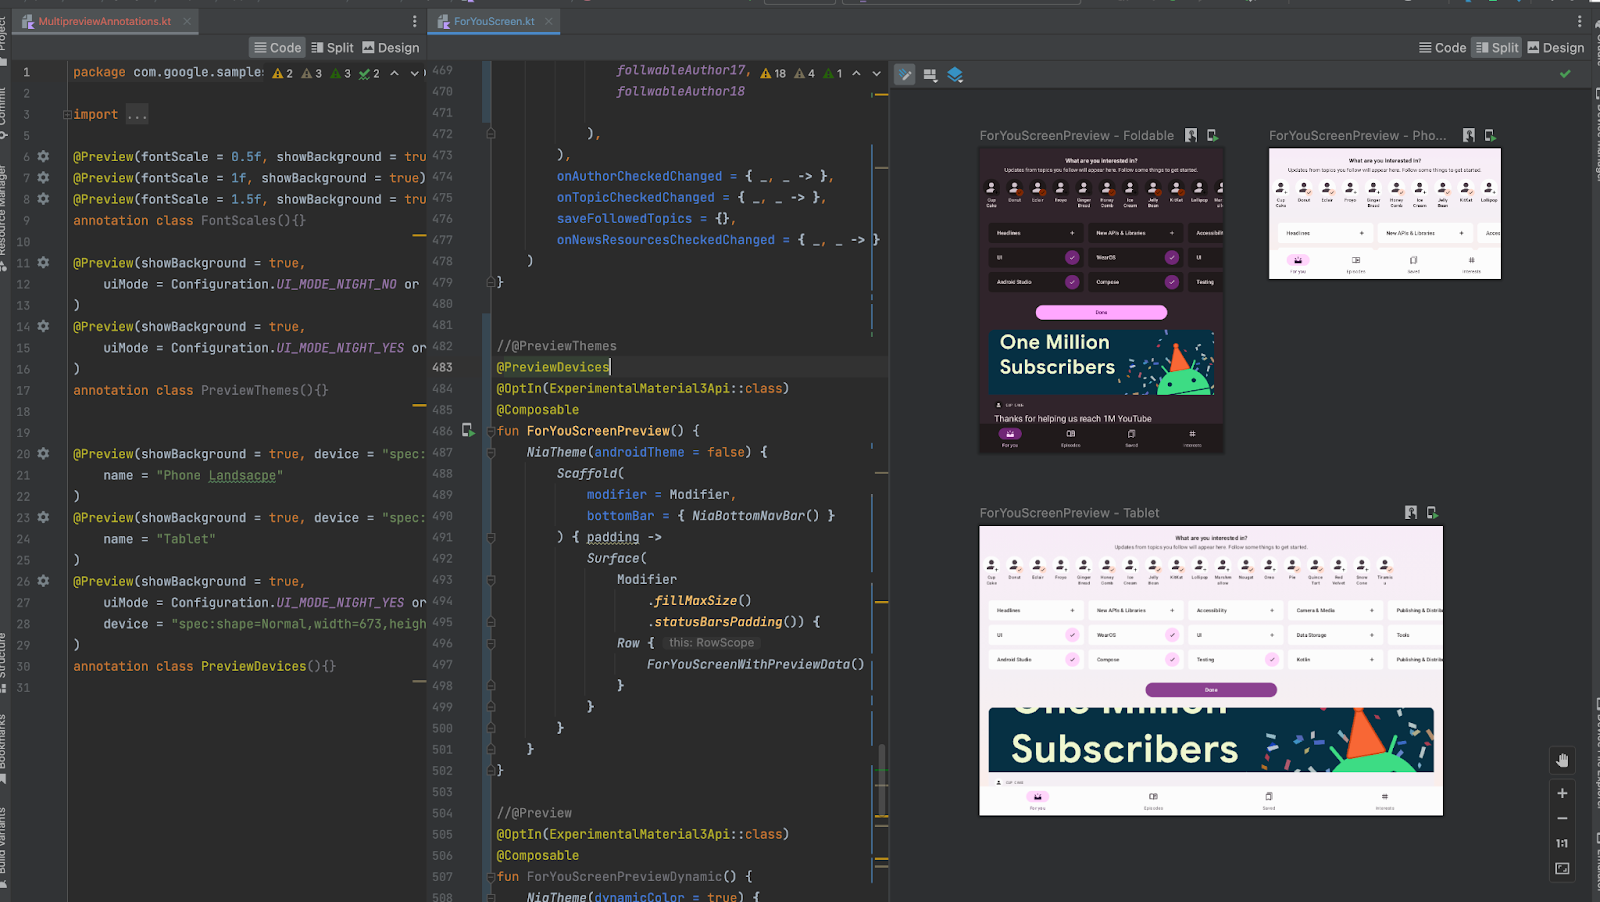
\includegraphics[scale=0.3]{android_studio_interface.png}
    \caption{Razvojno okruženje Android Studia}
\end{figure}
\\
\subsection{Neki dodatni alati Android Studia}
Alat AVD Manager (Android virtualni uređaj) je uključen u Android Studio i u osnovi je emulator koji omogućava pokretanje Android aplikacija na računaru. Zbog toga je vrlo koristan alat jer omogućava brzo testiranje aplikacija bez potrebe za instaliranjem na fizičke uređaje. Pored toga, omogućava simulaciju različitih veličina ekrana, specifikacija, verzija Androida ... Sve ovo i još više omogućava vam optimizaciju aplikacije za njeno izvršavanje na bilo kojem uređaju.

\begin{figure}[ht!]
    \centering
    \includegraphics[scale=0.2]{AVD_manager.png}
    \caption{AVD manager}
\end{figure}

Android Debug Bridge (ADB) je još jedan od korisnih alata Android Studia. U suštini, ovaj alat omogućava terminalni interfejs za interakciju sa telefonom. Kako je Android platforma bazirana na Linuxu, terminalni pristup je jedini način dobijanja admin pristupa. ADB omogućuje most između uređaja i kompjutera.

\begin{figure}[ht!]
    \centering
    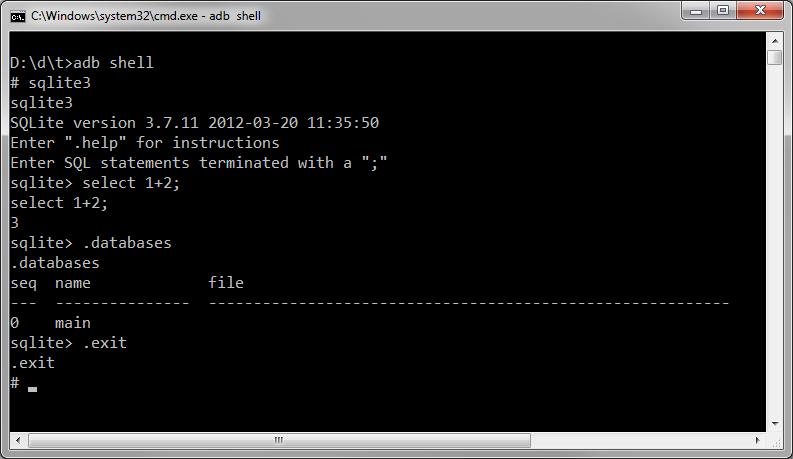
\includegraphics[scale=0.1]{adb.png}
    \caption{Android Debug Bridge}
\end{figure}


\section{Unity 3D}

\end{document}
